\documentclass[a4paper,12pt]{report}
\usepackage[T2A]{fontenc}
\usepackage[utf8]{inputenc}
\usepackage[english,russian]{babel}
\usepackage{graphicx}
\usepackage{wrapfig}
\usepackage{mathtext} 				% русские буквы в фомулах
\usepackage{amsmath,amsfonts,amssymb,amsthm,mathtools} % AMS
\usepackage{icomma} % "Умная" запятая: $0,2$ --- число, $0, 2$ --- перечисление
\usepackage{capt-of}
\usepackage{appendix}
\usepackage{multirow}
\usepackage{hyperref}
\usepackage{floatrow}
\usepackage[left=2cm,right=2cm,
    top=2cm,bottom=2cm,bindingoffset=0cm]{geometry}
\usepackage{multicol} % Несколько колонок
\usepackage{gensymb}
\title{Отчёт по лабораторной работе № 5.8.1. 

Определение постоянных Стефана-Больцмана и Планка из анализа теплового излучения накаленного тела.}
\author{Плюскова Н.А. Б04-004 }
\date{\today}
\begin{document}
\maketitle
\section*{1. Аннотация}
В данной работе был проверен закон Стефана-Больцмана, вычислены постоянная планка и константа Стефана-Больцмана.


\section*{2. Теоретические сведения}
Для измерения температуры разогретых тел, удалённых от наблюдателя, применяют методы оптической пирометрии, основанные на использовании зависимости испускательной способности исследуемого тела от температуры. Различают три температуры, функционально связанные с истинной термодинамической температурой и излучательной способностью тела: радиационную $T_{rad}$, цветовую $T_{col}$ и яркостную $T_b_r$. \par
В работе измеряется яркостная температура. \textbf{Яркостная температура} - это температура абсолютно чёрного тела, при которой его спектральная испускательная способность равна спектральной испускательной способности исследуемого тела при той же длине волны.
 Измерение яркостной температуры раскалённого тела производится при помощи оптического пирометра с исчезающей нитью, основанного на визуальном сравнении яркости раскалённой нити с яркостью изображения исследуемого тела. \par
Яркостная температура тела всегда ниже его термодинамической температуры. Это связано с тем, что любое нечёрное тело излучает меньше, чем АЧТ при той же температуре. Зависимость между яркостной и термодинамической температурами вольфрама приведена на рис. 1

\begin{figure}[h]
    \centering
    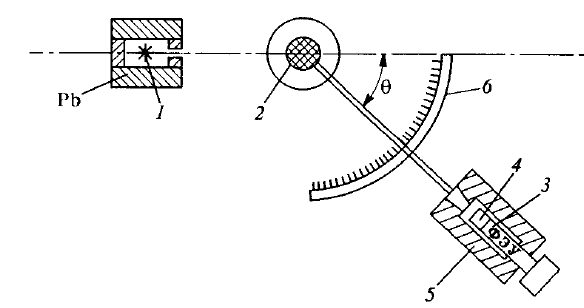
\includegraphics[width=10cm]{fig2.PNG}
    \caption{График зависимости $T = f(T_b_r)$ для вольфрам}
    \label{fig:vac}
\end{figure}

По результатам измерений мощности излучения вольфрамовой нити можно судить о справедливости закона Стефана-Больцмана. Если бы нить излучала как АЧТ, то баланс потребляемой и излучаемой энергии определялся бы соотношением 
\begin{equation}
    W = \sigma S (T^4 - T_0^4),
\end{equation}
где $W$ - потребляемая нитью электрическая мощность, $S$ - площадь излучающей поверхности нити, $T$ - температура нити, $T_0$ - температура окружающей среды. Однако вольфрамовая нить излучает как серое тел, и излучение её ослаблено по сравнению с АЧТ в $\varepsilon_T$ раз для любой волны при данной температуре тела Т. Тогда предположив, что нить излучает как серое тело и с учётом того, что $T_0 \ll T$, выражение (1) можно переписать в виде
\begin{equation}
    W = \varepsilon_T S \sigma T^4
\end{equation}
В справедливости закона Стефана-Больцмана можно убедиться, построив график зависимости $W(T)$ в логарифмическом масштабе и по углу наклона определить показатель степени $n$ исследуемой температурной зависимости. В пределах погрешности показатель степени должен быть близок к четырём. \par
Также из формулы (2) можно определить постоянную Стефана-Больцмана.

\section*{3. Экспериментальная установка}

\begin{figure}[h]
    \centering
    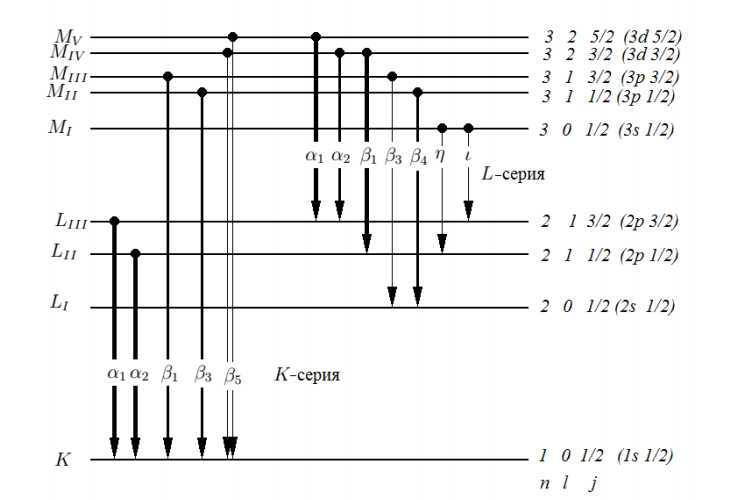
\includegraphics[width=11cm]{fig1.PNG}
    \caption{Схема экспериментальной установки: 1 - блок питания; 2 - тумблер включения питания образцов; 3 - тумблер нагрева нити пирометра; 4 - кнопка "Нагрев нити"; 5 - кнопка "охлаждение нити"; 6 - тумблер переключения образцов; 7 - регулятор мощности нагрева образцов; 8 - окуляр пирометра; 9 - корпус пирометра; 10 - объектив пирометра; 11 - переключение диапазонов; 12 - ручка смещения красного светофильтра; 13 - регулировочный винт; 14 - вольтметр (напряжение на лампе накаливания); 15 - амперметр (ток через образцы); 16 - вольтметр в цепи термопары; 17 - модель АЧТ; 18 трубка с кольцами из материалов с различной излучательной способностью; 19 - лампа накаливания; 20 - неоновая лампочка}
    \label{fig:vac}
\end{figure}

Исследуемые в работе образцы:
\begin{itemize}
    \item \textbf{модель абсолютно чёрного тела} - керамическая трубка, закрытая с одного конца и окружённая для теплоизоляции внешним кожухом. Температура в трубке измеряется с помощью термопары хромель-алюмель
    \item \textbf{керамическая трубка с набором колец из различных материалов}, нагреваемая изнутри нихромовой спиралью. Материалы колец имеют различную излучательную способность
    \item \textbf{вольфрамовая нить электрической лампочки}
\end{itemize}

\section*{4. Ход работы}
\subsection*{4.1 Изучение работы оптического пирометра}
С помощью пирометра измерим температуру модели АЧТ и сравним со значением температуры, измеренной при помощи термопарного термометра:
\begin{table}[H]
\begin{tabular}{|c|c|c|c|}
\hline
$T_{\text{пирометра}}, C^{o}$ & $V_{\text{термопары}}$, мВ & $T_{\text{АЧТ}}, C^{o}$ & Разность   значений, $\%$ \\ \hline
947        & 37,03     & 903  & 4,9                     \\ \hline
957        & 37,56     & 916  & 4,5                     \\ \hline
967        & 37,82     & 922  & 4,9                     \\ \hline
977        & 38,13     & 930  & 5                       \\ \hline
\end{tabular}
\end{table}

Заметим, что значения температуры, измеренной при помощи термопары и пирометра сходятся в пределах 5$\%$.
\subsection*{4.2 Измерение яркостной температуры накаленных тел}
С помощью пирометра необходимо было снять температуру трех колец из различных материалов, находившихся на керамической трубке. Однако кольца были нагреты до температуры, которую невозможно было измерить пирометром, т.к. она находилась за пределом измерений прибора.
\subsection*{4.3 Проверка закона Стефана-Больцмана}
Измерим яркостную температуру лампы накаливания и переведем полученный результат в абсолютную температуру с помощью графика зависимости $T(T_{br})$ для вольфрамовой нити:

\begin{figure}[H]
    \centering
    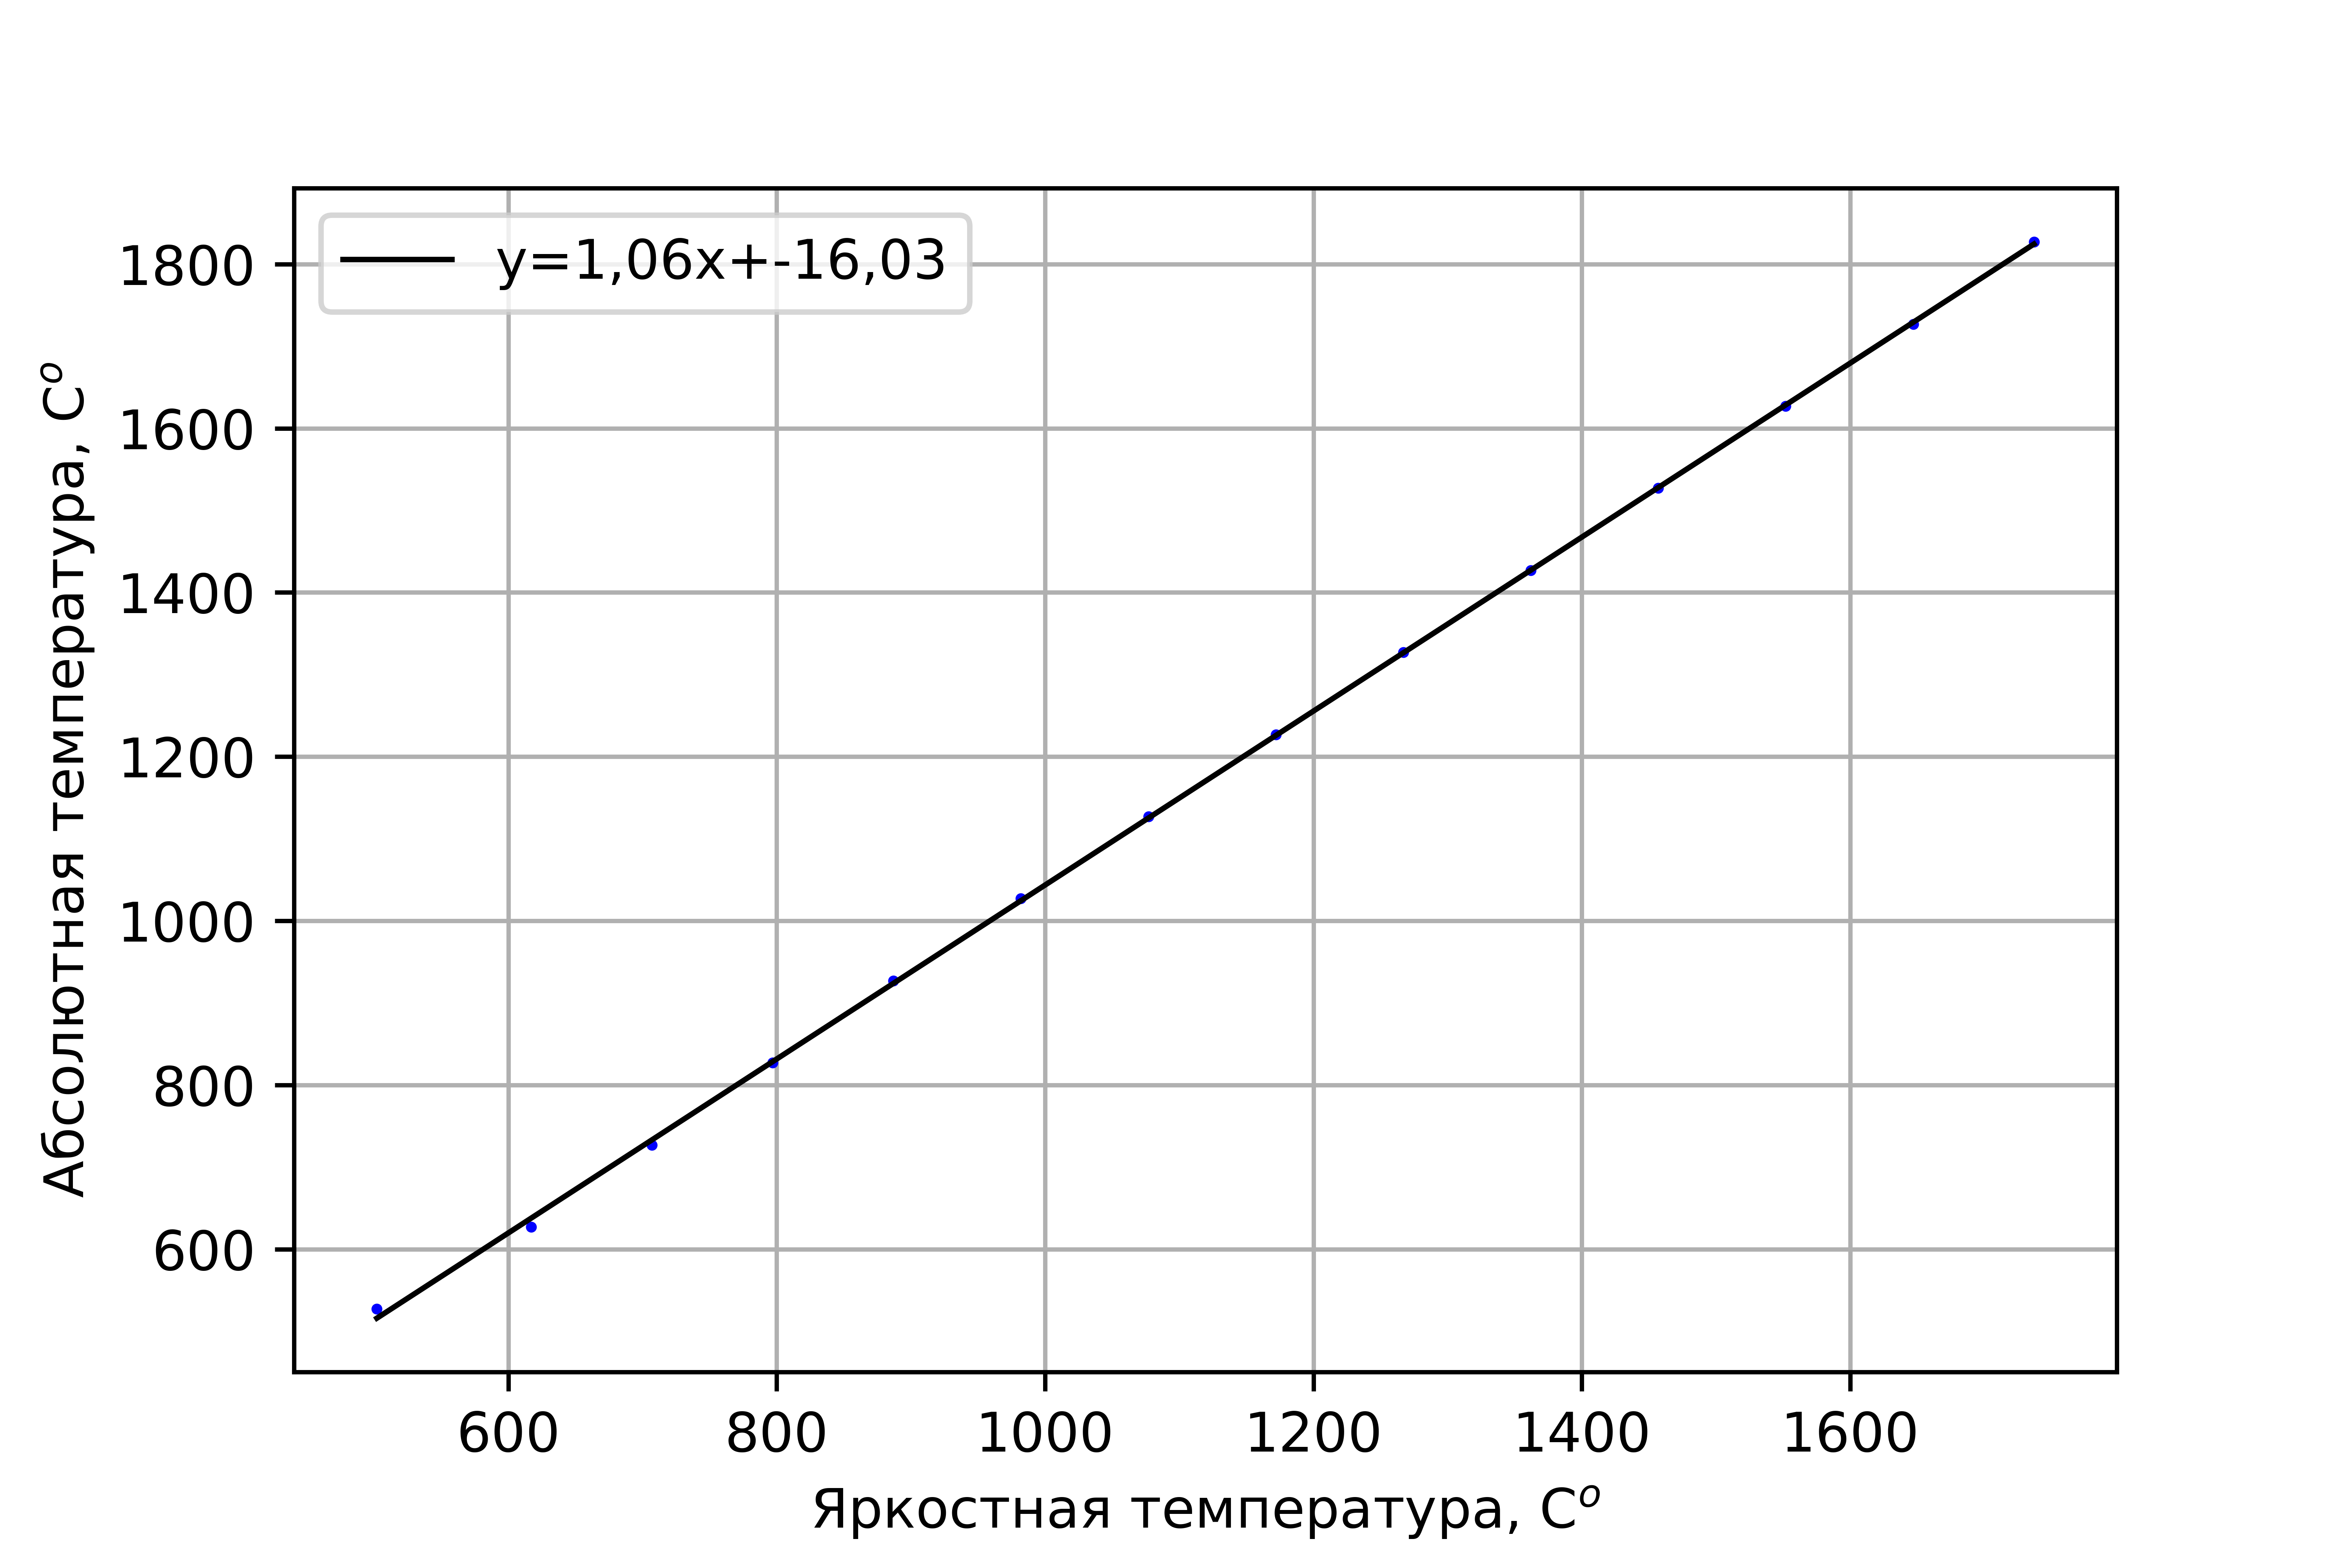
\includegraphics[width=14cm]{T(T_yar).png}
    \caption{$T(T_b_r)$ для вольфрама}
    \label{fig:vac}
\end{figure}

\begin{table}[H]
\begin{tabular}{|c|c|c|c|c|c|c|c|}
\hline
$I$, мА & $\sigma_{I}$, мА          & $V$, В  & $\sigma_{V}$, В               & $T_{br}, C^{o}$ & $T, C^{o}$ & $W$, мВт  & $\sigma_{W}$,мВт \\ \hline
433   & \multirow{12}{*}{1} & 1,348 & \multirow{12}{*}{0,001} & 800        & 832      & 583,68  & 1,42       \\ \cline{1-1} \cline{3-3} \cline{5-8} 
457   &                     & 1,528 &                         & 900        & 938      & 698,30  & 1,59       \\ \cline{1-1} \cline{3-3} \cline{5-8} 
473   &                     & 1,658 &                         & 1000       & 1044     & 784,23  & 1,72       \\ \cline{1-1} \cline{3-3} \cline{5-8} 
522   &                     & 2,087 &                         & 1100       & 1150     & 1089,41 & 2,15       \\ \cline{1-1} \cline{3-3} \cline{5-8} 
578   &                     & 2,595 &                         & 1200       & 1255     & 1499,91 & 2,66       \\ \cline{1-1} \cline{3-3} \cline{5-8} 
621   &                     & 3,018 &                         & 1300       & 1361     & 1874,18 & 3,08       \\ \cline{1-1} \cline{3-3} \cline{5-8} 
685   &                     & 3,681 &                         & 1400       & 1467     & 2521,49 & 3,74       \\ \cline{1-1} \cline{3-3} \cline{5-8} 
772   &                     & 4,666 &                         & 1500       & 1573     & 3602,15 & 4,73       \\ \cline{1-1} \cline{3-3} \cline{5-8} 
822   &                     & 5,264 &                         & 1600       & 1679     & 4327,01 & 5,33       \\ \cline{1-1} \cline{3-3} \cline{5-8} 
899   &                     & 5,243 &                         & 1700       & 1785     & 4713,46 & 5,32       \\ \cline{1-1} \cline{3-3} \cline{5-8} 
934   &                     & 6,73  &                         & 1800       & 1891     & 6285,82 & 6,79       \\ \cline{1-1} \cline{3-3} \cline{5-8} 
1013  &                     & 7,828 &                         & 1900       & 1997     & 7929,76 & 7,89       \\ \hline
\end{tabular}
\caption{Измерения для проверки закона Стефана-Больцмана}
\end{table}

Построим график W=f(T):

\begin{figure}[H]
    \centering
    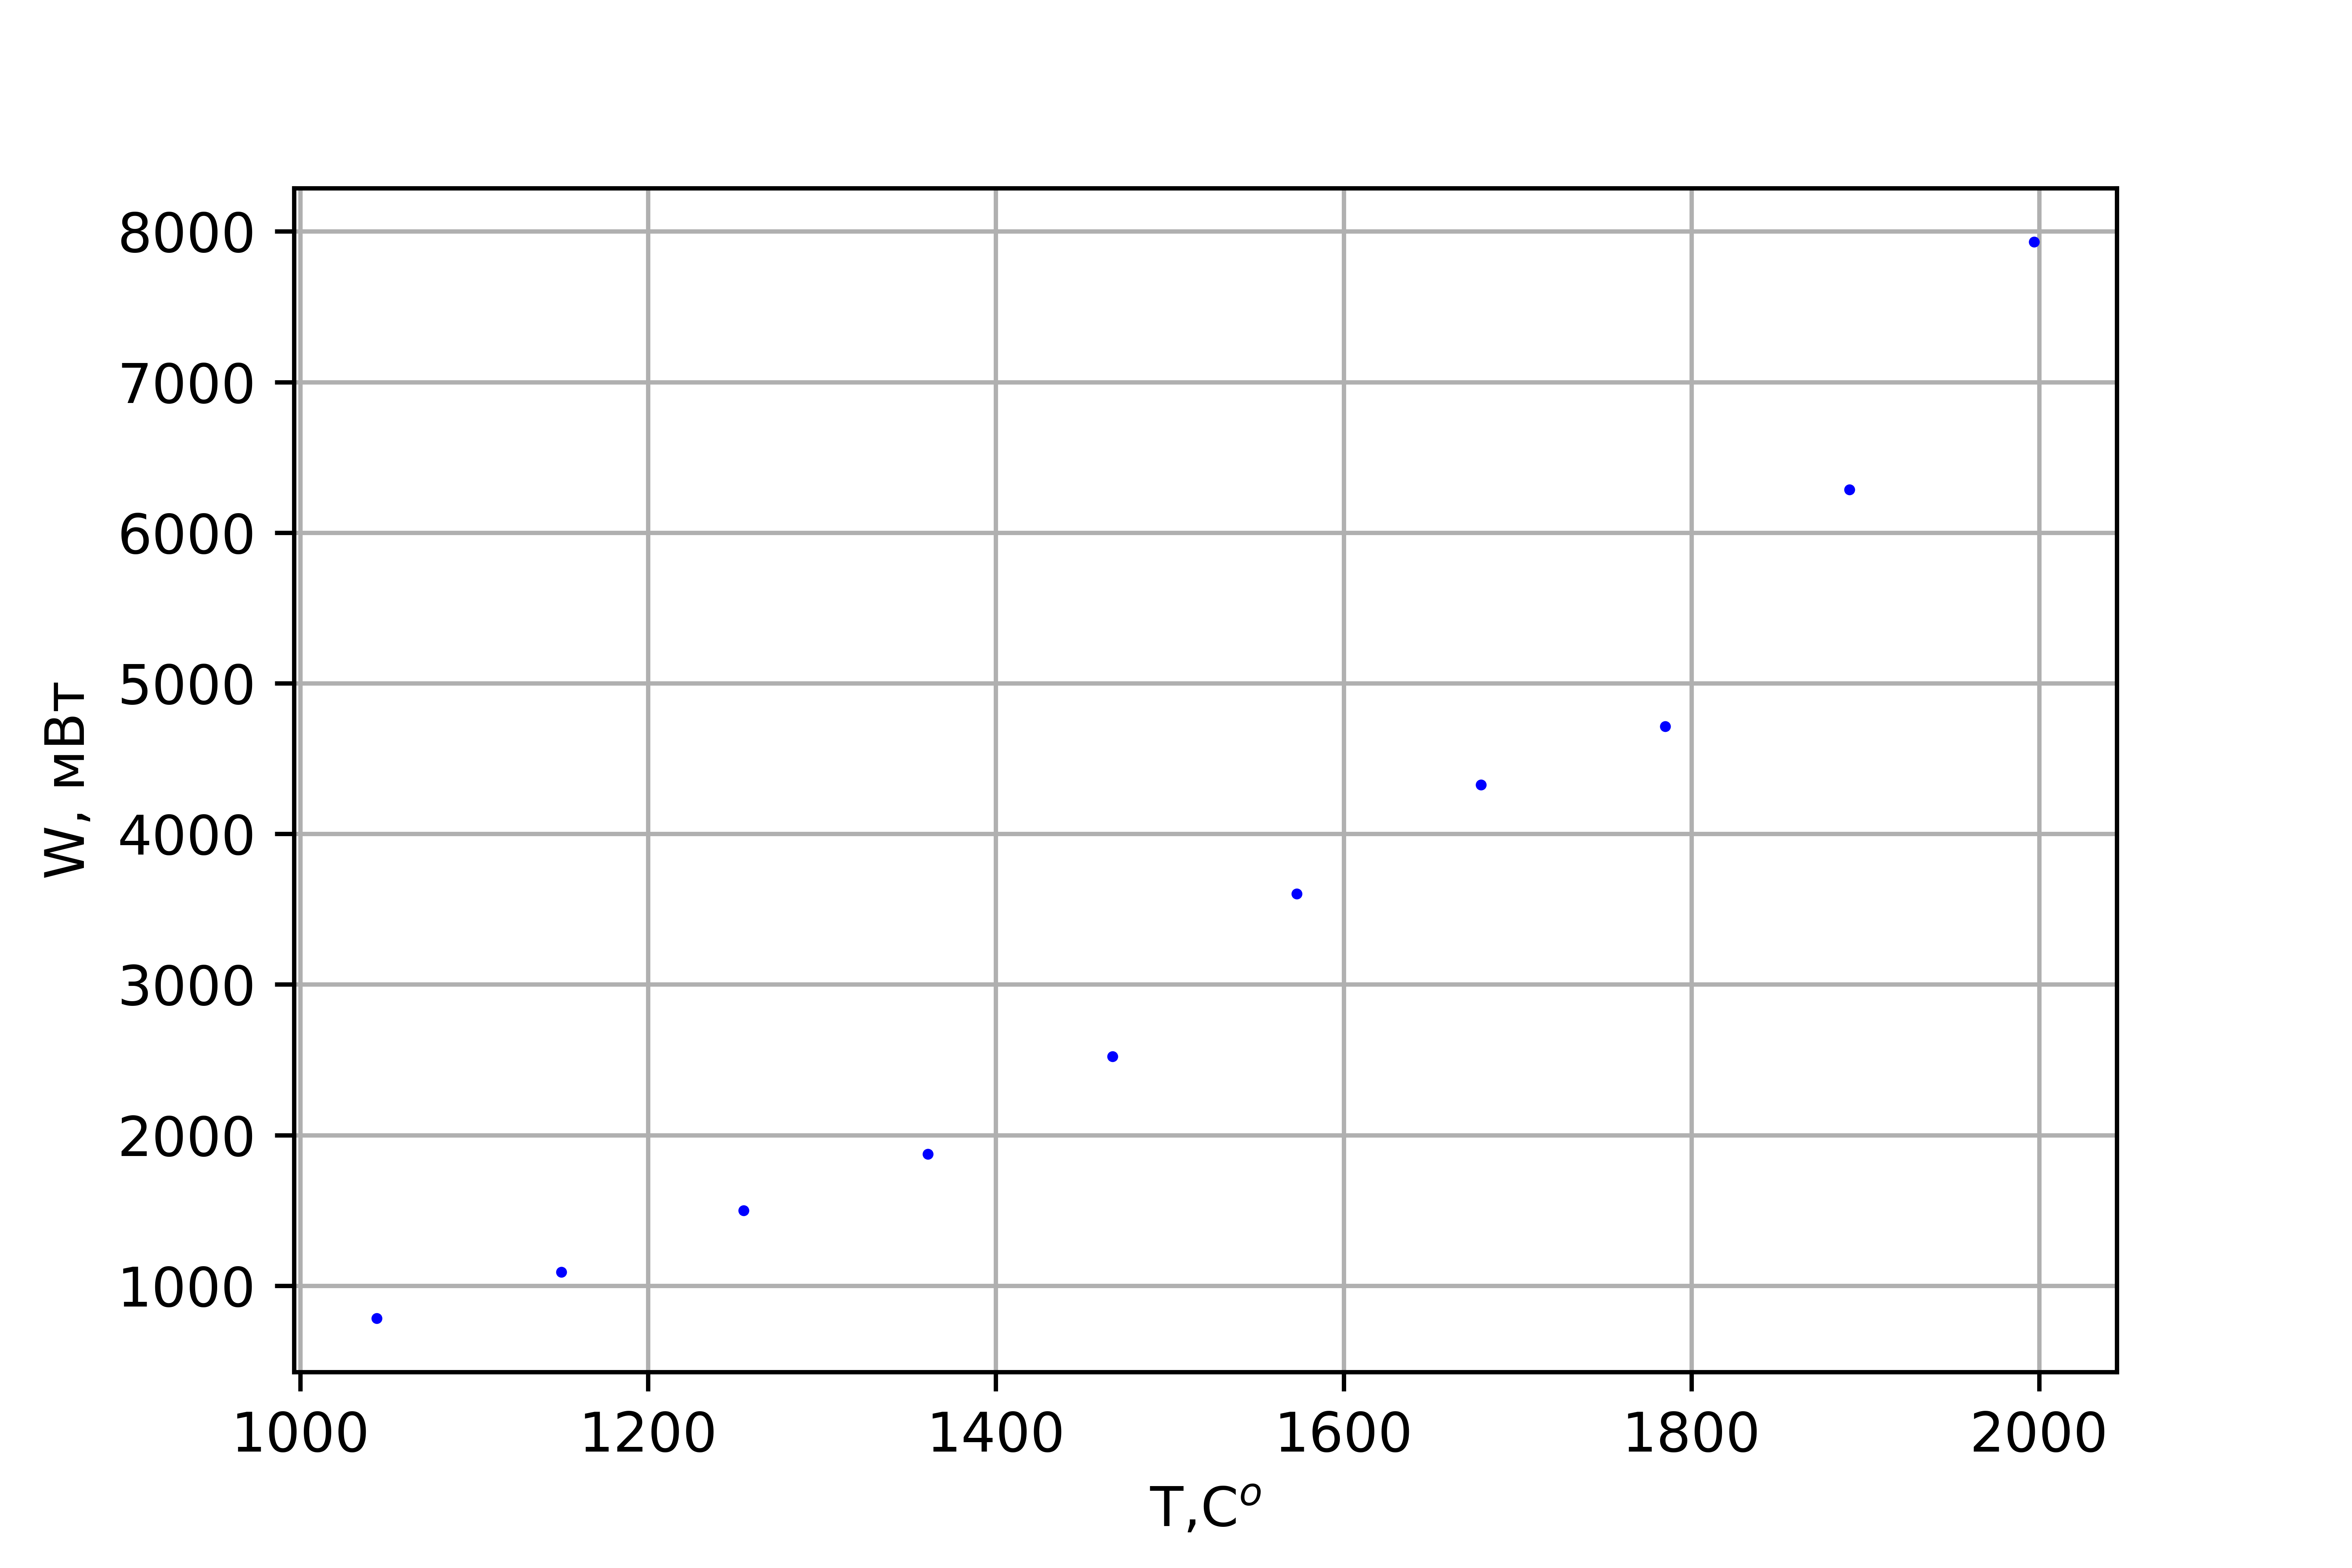
\includegraphics[width=14cm]{W(T).png}
    \caption{W=f(T)}
    \label{fig:vac}
\end{figure}

Построим тот же график в логарифмическом масштабе, чтобы проверить закон Стефана-Больцмана:

\begin{figure}[H]
    \centering
    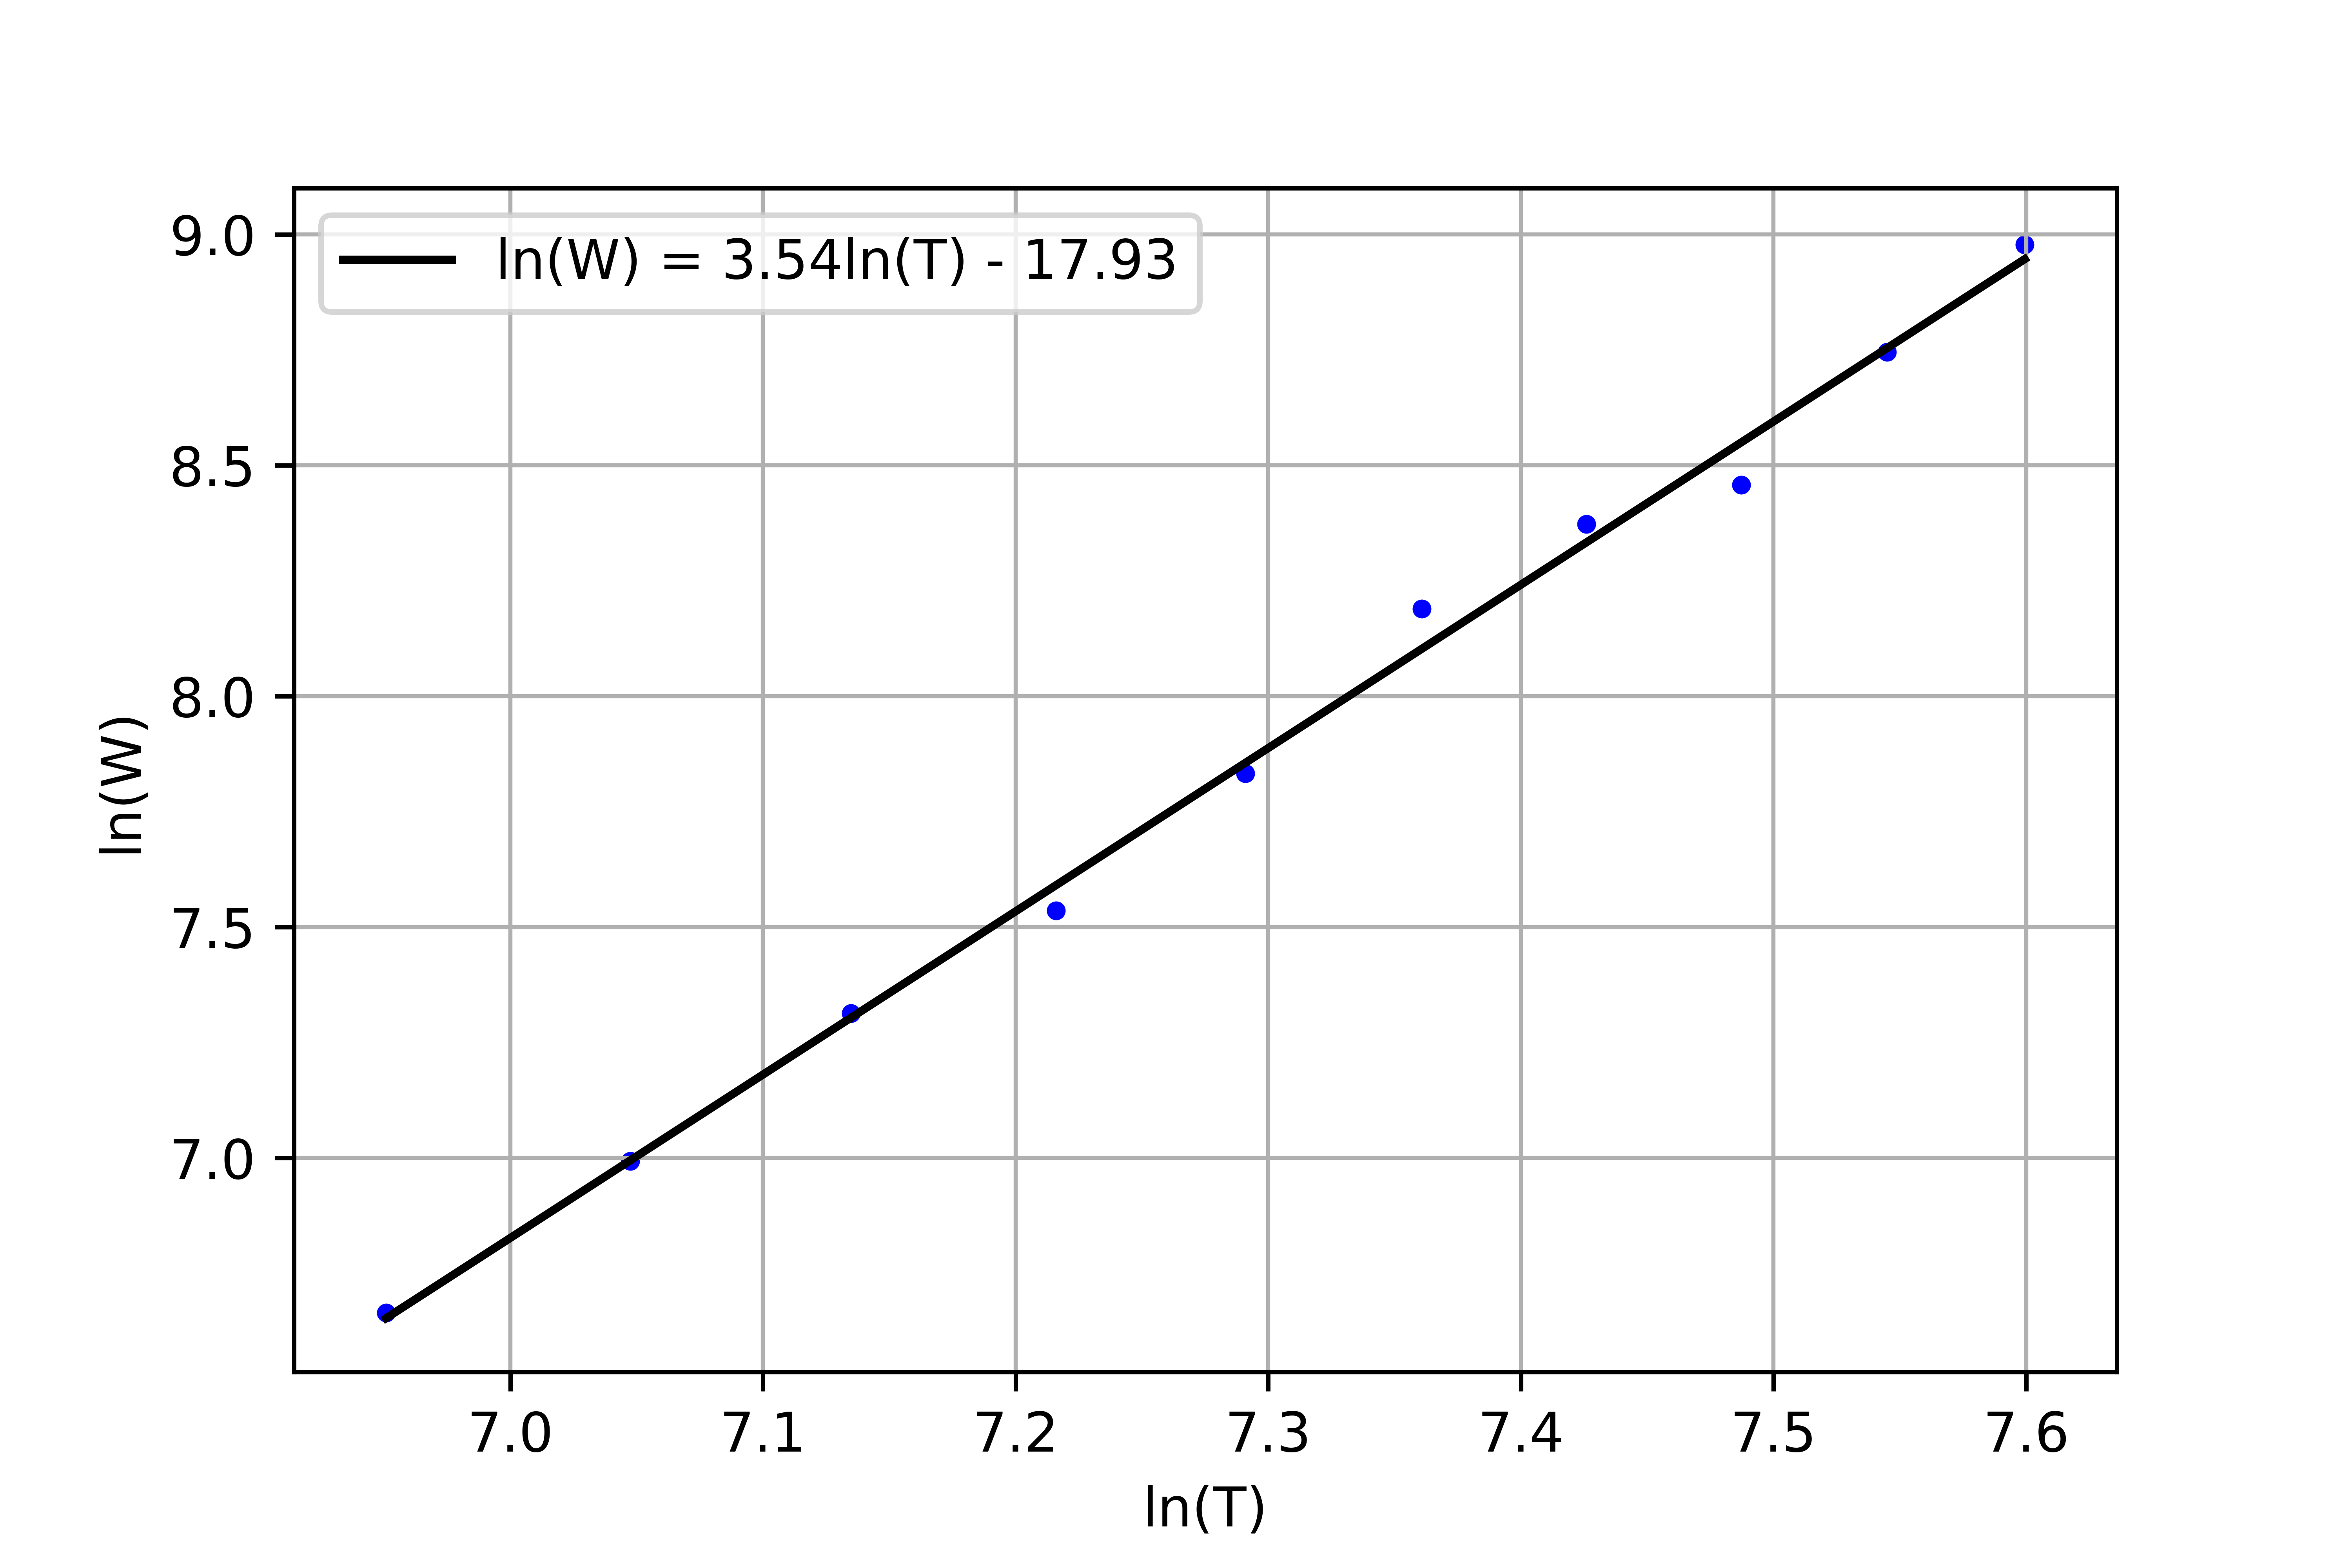
\includegraphics[width=14cm]{lnW(lnT).png}
    \caption{$ln(W) = ln(\varepsilon_{T}B)+nlnT$}
    \label{fig:vac}
\end{figure}

Из график видно, что коэффициент наклона прямой, соответствующий степени $n$ в законе Стефана-Больцмана примерно равен 4, что сходится с теоретическими данными.

Найдем величину константы Стефана-Больцмана по формуле:
\begin{equation*}
    \sigma = \frac{W}{\varepsilon_{T}ST^{4}}
\end{equation*}

Определим $\varepsilon_{T}$ по нижеприведенному графику для каждой температуры, выше 1700 К:

\begin{figure}[H]
    \centering
    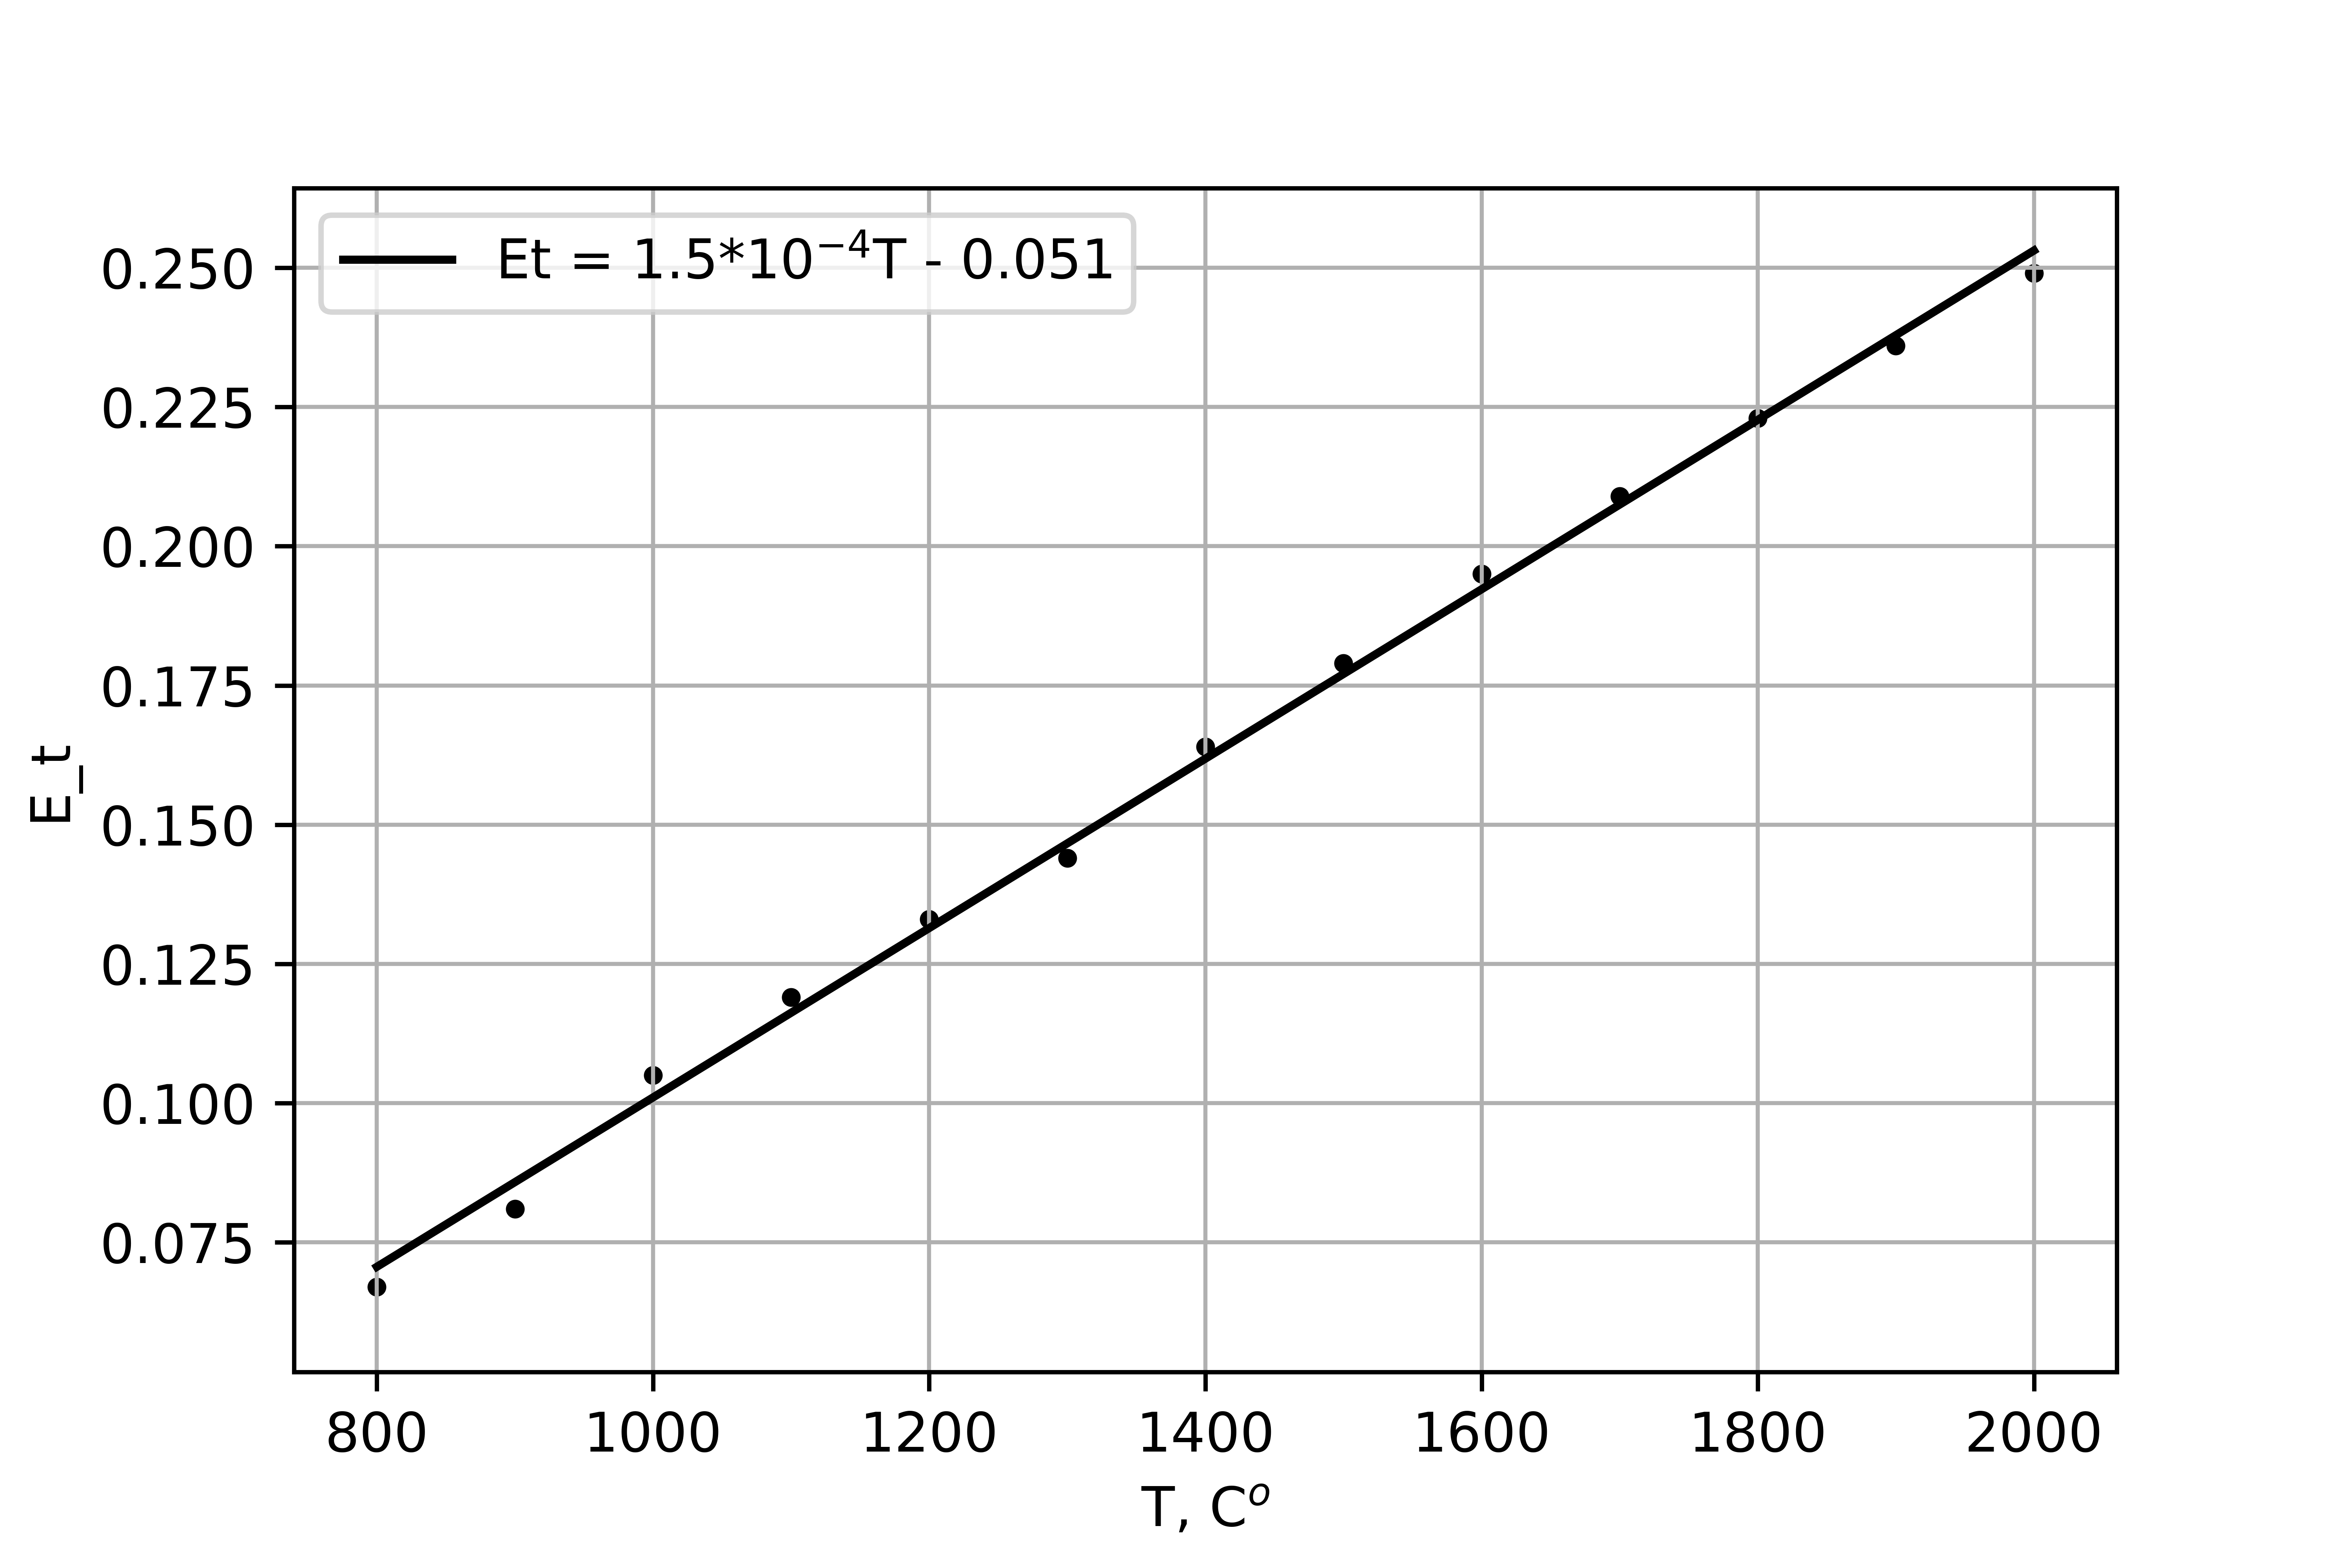
\includegraphics[width=14cm]{Et(T).png}
    \caption{$\varepsilon_{T}(T)$}
    \label{fig:vac}
\end{figure}

\begin{table}[H]
\begin{tabular}{|c|c|c|c|c|c|c|}
\hline
$W$, мВт  & $\sigma_{W}$,мВт & $\varepsilon_{T}$    & $T$, K & $\sigma_{T}$,K             & $\sigma \cdot 10^{-12}$, $\frac{\text{Вт}}{\text{см}^{2}\cdot \text{К}^{4}}$& $\sigma_{\sigma} \cdot10^{-12}$, $\frac{\text{Вт}}{\text{см}^{2}\cdot \text{К}^{4}}$ \\ \hline
3602,15 & 4,73       & 0,188 & 1846 & \multirow{5}{*}{1} & 4,580                               & 0,012                                   \\ \cline{1-4} \cline{6-7} 
4327,01 & 5,33       & 0,204 & 1952 &                    & 4,056                               & 0,010                                   \\ \cline{1-4} \cline{6-7} 
4713,46 & 5,32       & 0,22  & 2058 &                    & 3,316                               & 0,007                                   \\ \cline{1-4} \cline{6-7} 
6285,82 & 6,79       & 0,237 & 2164 &                    & 3,358                               & 0,004                                   \\ \cline{1-4} \cline{6-7} 
7929,76 & 7,89       & 0,253 & 2270 &                    & 3,278                               & 0,003                                   \\ \hline
\end{tabular}
\end{table}

Получим $\sigma \approx (3,717 \pm 0,012) \cdot 10^{-12}$ $\frac{\text{Вт}}{\text{см}^{2}\cdot \text{К}^{4}}$. Заметим, что полученное значение константы Стефана-Больцмана сходится по порядку с теоретическим.

По найденному значению $\sigma$ найдем постоянную планка по формуле:

\begin{equation*}
    h = \sqrt[3]{\frac{2\pi^{5}{k_{\text{б}}^4}}{15c^2\sigma}} = (1,64 \pm 0,02)\cdot 10^{-27} \text{ эрг}\cdot\text{с}
\end{equation*}

\subsection*{4.4 Измерение "яркостной температуры" неоновой лампочки}
Прикоснувшись к лампочке, можно заметить, что ее температура примерно равна комнатной и отличается от ее "яркостной температуры". Причина в том, что неоновая лампочка не является моделью АЧТ, а ее излучение носить иной характер (переход электронов между энергетическими уровнями)


\section*{5. Выводы}
В ходе работы был проверен закон Стефана-Больцмана, найдена степень $n\approx 4$, что совпадает с теоретическими данными, также получено значение константы Стефана-Больцмана $\sigma \approx (3,717 \pm 0,012) \cdot 10^{-12}$ $\frac{\text{Вт}}{\text{см}^{2}\cdot \text{К}^{4}}$, по порядку совпадающее с теоретическим. Также была вычислена постоянная Планка $h = (1,64 \pm 0,02)\cdot 10^{-27}$ эрг$\cdot$с. Полученное значение $h$ по порядку совпадает с теоретическим.

\end{document}
